\documentclass[report.tex]{subfiles}

\begin{document}

    \section*{\centering Introduction}

    Reinforcement learning has made huge advances in the last couple of years, in particular with games such as when AlphaGo from Google DeepMind won against Lee Sedol in the game Go in 2016 \cite{silver2016mastering}. It has also been possible to learn the computer to play Atari games \cite{mnih2013playing} and this year at the largest eSports event in the world, the International 2017, OpenAI demonstrated that reinforcement learning can be used to defeat some of the best players in Dota 2 in 1 versus 1. \footnote{https://blog.openai.com/dota-2/}

    Reinforcement is another large area in machine learning alongside supervised and unsupervised learning. The idea behind reinforcement learning is learning by interacting with an environment, which is how learning in nature happens very often. A child putting its hands on a hot stove will quickly feel a painful sensation and remember that was a terrible idea, and ultimately learn from it. Learning can also have positive effects such as when a mouse reaches the end of the labyrinth and finds a piece of cheese.

    Reinforcement learning is a computational framework to this kind of learning by having a so called \textit{agent} interact with an environment and learn how to respond to different scenarios. The goal is to create learning methods that can learn an optimal \textit{policy}, a mapping from the current sensory input to a decision in the form of an action, according to a behavior we want it to achieve. That might be from learning the computer to play tic-tac-toe to more complex behavior such as flying a helicopter where the agent do not posses full control of the environment.

    \subsection*{Snake}

    This report is meant to look at some of the basic fundamental building blocks of reinforcement learning and in order to do so we need a problem that we would like to solve. Snake is an old game\footnote{https://en.wikipedia.org/wiki/Snake\_(video\_game)} and has been around for a long time and there are many variations of it. In this report, the game is played out as simple as possible with only one player and no obstructing environment. The goal of the game is that you play as a snake by controlling the head and the aim is to eat as many apples as possible without colliding with either the snake's body or the edges of the game board. The difficulty is that each time you eat an apple your body becomes longer and thus larger portion of the game board is covered by it. In order to reduce the state space the game board is 5x5 which can be seen in figure \ref{fig:snake}.

    \begin{figure}[H]
        \centering
        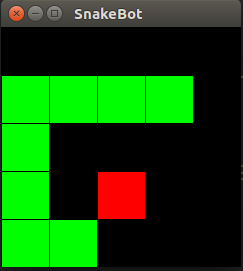
\includegraphics[scale=0.5]{./images/snake}
        \label{fig:snake}
        \caption{5x5 board of Snake where the snake consists of the green parts and the red part is the apple.}
    \end{figure}

    \subsection*{Questions}

    \begin{enumerate}
        \item Is the state representation important for learning?
        \item Is it important for the reward function to reinforce behavior we want the agent to learn?
        \item Is punishing bad behavior equivalent to reinforcing good behavior?
        \item Is it better if the reward function combines reinforcement and punishment?
    \end{enumerate}

\end{document}
